\subsection*{Redigering}
Redigering inddeles i en boundary og en tilhørende controller, som det fremgår af \autoref{fig:Redigering}. 

\begin{figure} [H]
\centering
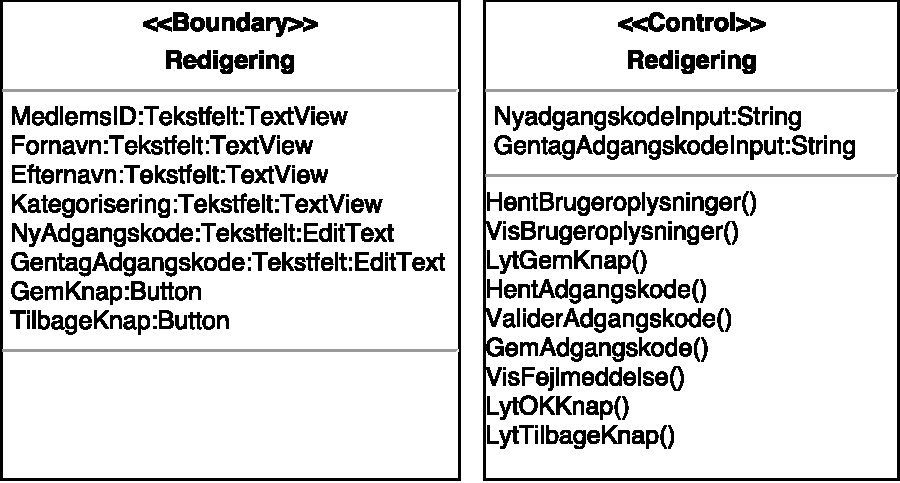
\includegraphics[width=0.7\textwidth]{figures/MVC/Redigering}
\caption{Designklasser for Redigering. Til venstre fremgår boundary og til højre controller for redigering.}
\label{fig:Redigering}
\end{figure}

\noindent
I grænsefladen for \textit{Redigering} opstilles tekstfelter af typen TextView for medlemsID, navn og kategorisering. Derudover opstilles tekstfelter, af typen EditText, for ny adgangskode og gentag adgangskode, hvor brugeren kan angive en ny adgangskode. Dertil er der en GemÆndringKnap, af typen Button. GemÆndringKnap indikerer ved tryk, at brugeren ønsker at gemme den nye adgangskode. 
Den tilhørende controller har metoderne Hent, Vis, Lyt, Valider, Gem og Fejlmeddelelse **BEKRÆFTELSE!***. Til disse klasser er der opstillet et sekvensdiagram, hvilket fremgår af \autoref{fig:SEKRedigering}.


\begin{figure} [H]
\centering
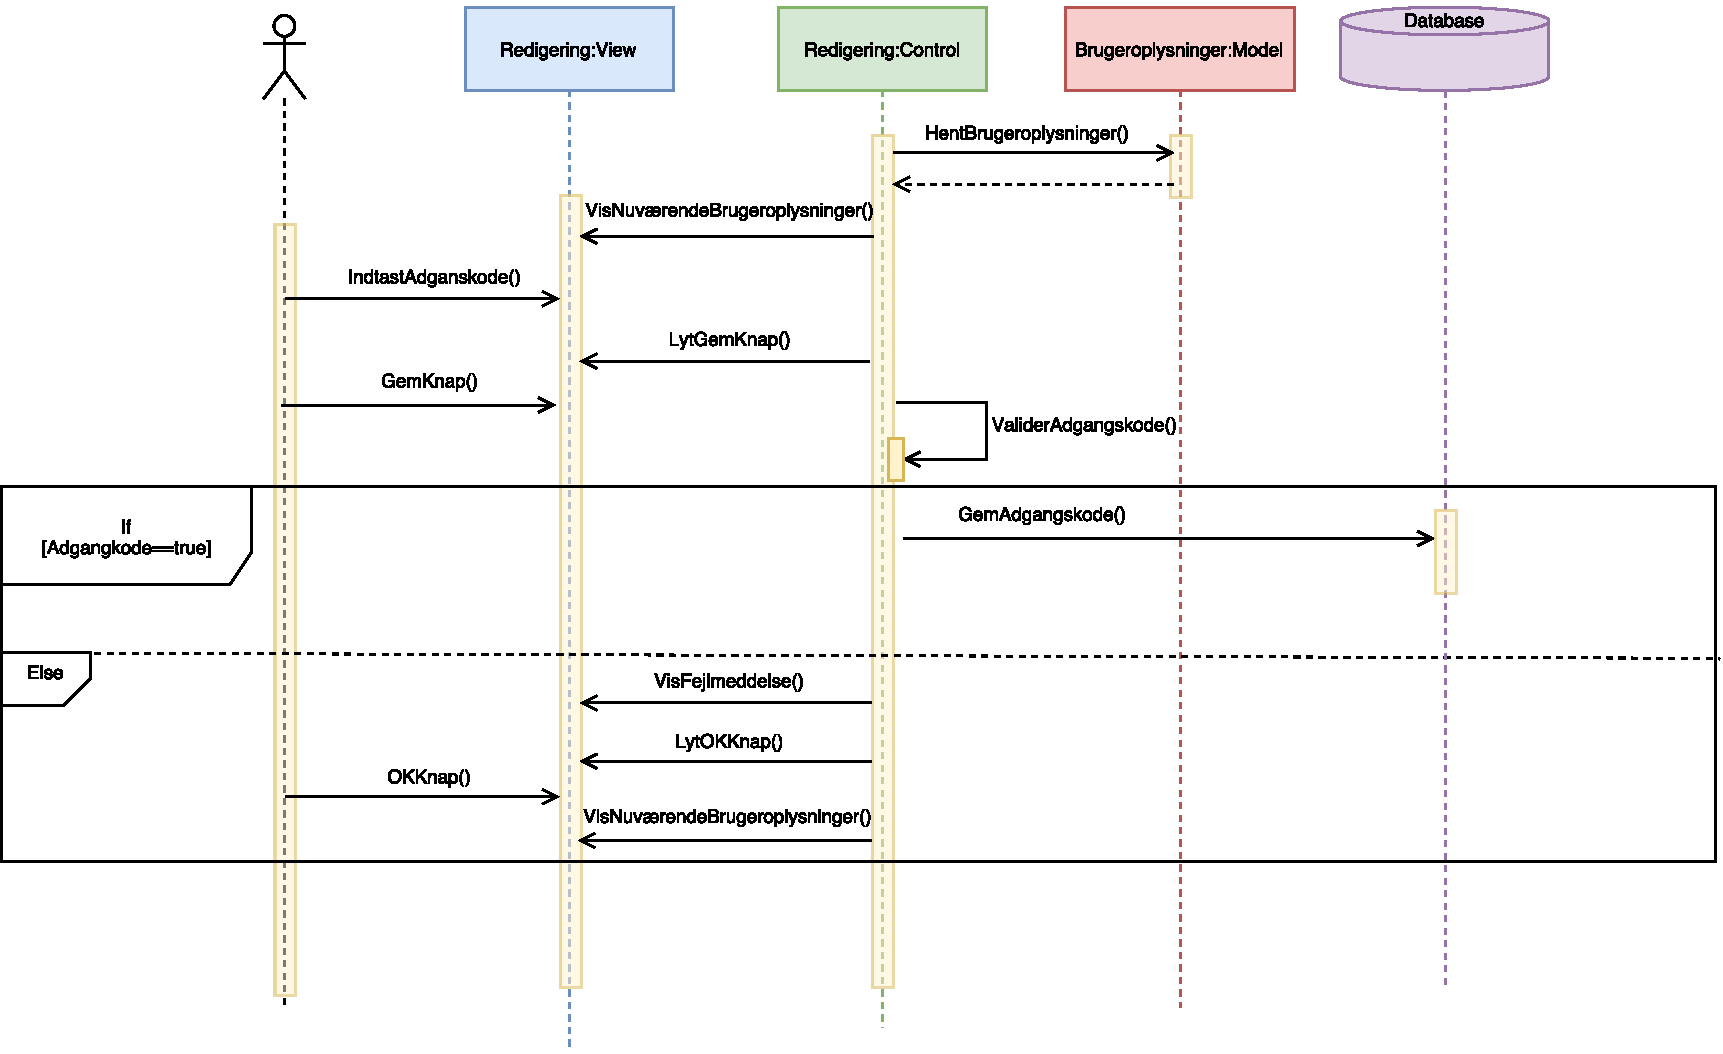
\includegraphics[width=1\textwidth]{figures/Sek/SEKRedigering}
\caption{Sekvensdiagram for redigering.}
\label{fig:SEKRedigering}
\end{figure}

\noindent
Controlleren \textit{Redigering} henter brugeroplysninger fra modellen \textit{Brugeroplysninger}. Disse oplysninger vises i grænsefladen \textit{Redigering}, hvortil brugeren kan se sin information. Fra denne grænseflade er det ligeledes muligt for brugeren at ændre sin adgangskode. Adgangskoden skal indtastes to gange for at sikre, at adgangskoden er identisk. Dertil skal adgangskoden være minimum 10 karakterer lang. Adgangskoden valideres, hvis adgangskoden overholder de førnævnte kriterier, gemmes denne direkte i \textit{Database} via dens controller.
Overholder adgangskoden derimod ikke kriterierne, vises en fejlmeddelelse i grænsefladen. Denne forsvinder efter kort tid, hvortil grænsefladen for redigering vises igen. 
